\documentclass[]{article}

\usepackage[english]{babel}
\usepackage[utf8]{inputenc}
\usepackage{amsmath}
\usepackage{graphicx}
\begin{document}

\title{Electronique II}
\author{Dylan Bourgeois}
\date{MT BA4}
\maketitle

\section{Introductions}
Cours d'électronique II, donné par Mme Lacour.
\section{Polarisation et Jonction PN}
\subsection{...}
A completer avec les notes.

\subsection{Diode Zener}
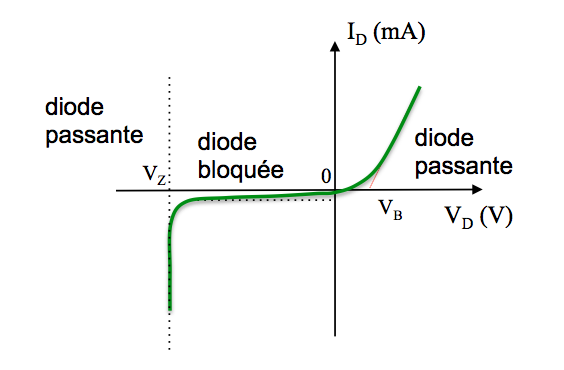
\includegraphics[scale=0.8]{zener_IV.png} 
\subsection{A retenir}

La polarisation d'une jonction PN modifie la distribution des charges à la surface:

-  \textbf{Polarisation directe} : les porteurs minoritaires sont injectés dans les "zones neutres"

- \textbf{Polarisation inverse} : les porteurs minoritaires sont arrachés dans les "zones neutres"

Caractéristique $I(V)$ de la diode PN : $$ I_D \approx I_s \exp{(\frac{qV_D}{nkT})} $$

Paramètres essentiels : $V_B , - I_s, r_d$

\section{Le transistor bipolaire}
\subsection{Structure du transistor}
\subsubsection{Le transistor}
Polarité indiquée par la flèche ($=$ direction du courant $I_E$)
Comporte trois électrodes :

- \textbf{Base} : électrode de commande.

- \textbf{Collecteur} : Relié au $\oplus$ de l'alimentation.

- \textbf{Emetteur} : draine les courants de base et de collecteur.

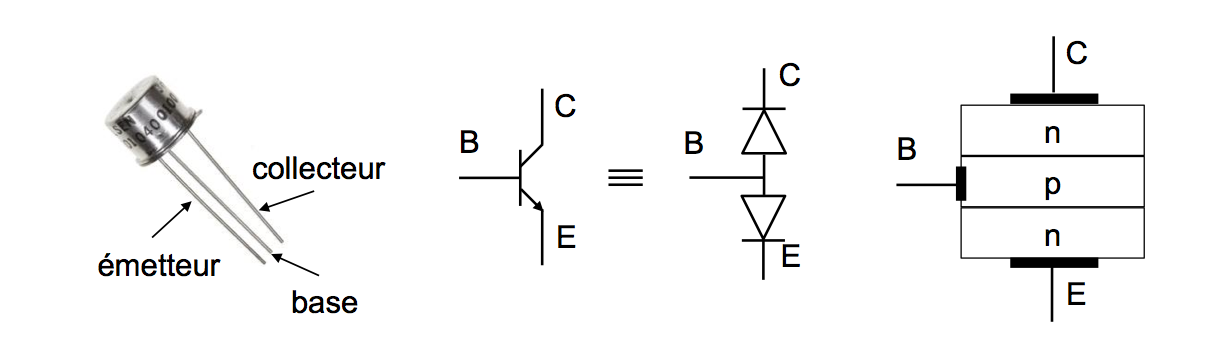
\includegraphics[scale=0.6]{transistor.png} 

\subsubsection{Transistor NPN}

\begin{itemize}
\item \textbf{Etats de fonctionnement} :\quad \quad
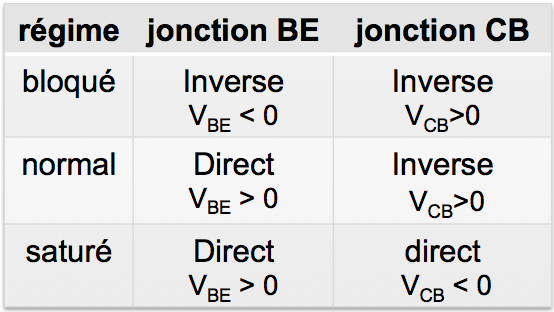
\includegraphics[scale=0.6]{npn_etats.png} 

\item \textbf{Fonctionnement normal} :
La "diode" BE est polarisée en mode direct, donc $V_{BE} > 0$. Les courants de diffusion sont des porteurs majoritaires : Trous de $B\rightarrow E$, $e^-$ de $E\rightarrow B$.
La "diode" BC est ploarisée en mode inverse, donc $V_{BC} <  0$.  Les courants de diffusion sont des porteurs minoritaires :  $e^-$ de $B\rightarrow C$.
Au final, une large portion d'$e^-$ se déplacent de $E\rightarrow C$, et un faible courant de trous se déplacent de $B \rightarrow E$.
\end{itemize}

\subsubsection{Les courants $I_B,I_E,I_C$}

Courant de collecteur (\textbf{NB} : ne dépend que de $V_{BE}$) : 
$$I_C = I_S \exp{(\frac{V_{BE}}{U_T}-1)}$$ 

Courant de base (avec $\beta$ le gain en courant, $50 < \beta < 200$) : 
$$ I_B = \frac{I_C}{\beta} $$

Courant d'émetteur : $$ I_E =  ( \frac{1}{\beta} + 1 ) I_S \exp{(\frac{V_{BE}}{U_T}-1)}$$

\subsubsection{Autres modes de fonctionnement}
\begin{itemize}
\item \textbf{Bloqué :}

Les deux jonctions BE et BC sont en mode inverse
Aucun courant ne circule
Le collecteur est isolé de l'émetteur (circuit ouvert) ($V_{CE} \rightarrow V_{CC}$)
$$ i_B = i_C = i_E = 0 $$
\item \textbf{Saturé :}

Le deux jonctions BE et BC sont en mode direct : $V_{BE} \sim 0.7V$ et $ V_{BC} \sim 0.7V$.
Diminution de $V_{CE} \rightarrow V_{CE,sat} \sim 0.2-0.3V$
Augmentation du courant de base $i_B$ jusqu'à $i_{B,sat} > \frac{i_{C,sat}}{\beta}$.
\end{itemize}

\subsubsection{A retenir}
En mode normal, les courants sont proportionnels entre-eux et au facteur $\exp{(\frac{V_{BE}}{V_T})}$. De plus $V_{BE}$ controle $I_C$ (effet transistor). Ce dernier est indépendant de $V_{BC}$ (isolation), mais est controlé via $I_B$.

\subsection{Caractéristiques I(V)}
\subsubsection{$I_C = f(V_{BE})$}
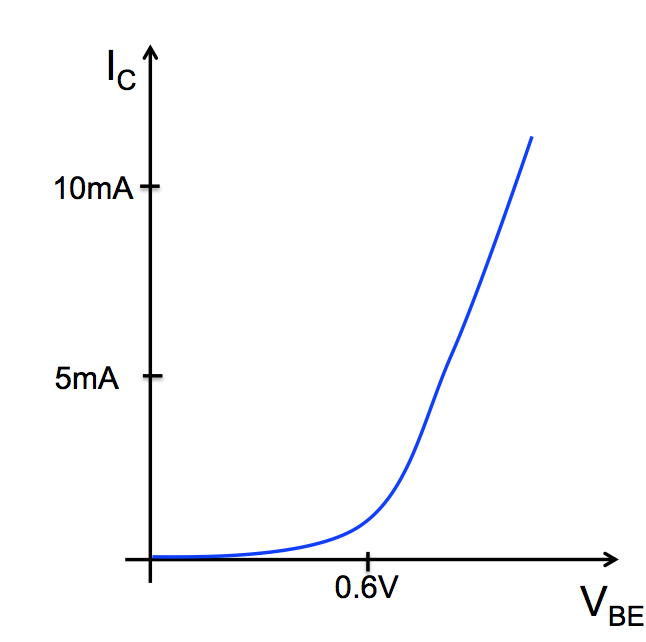
\includegraphics[scale=0.4]{Ic_Vbe.png}
\subsubsection{$I_C = f(I_B)$}
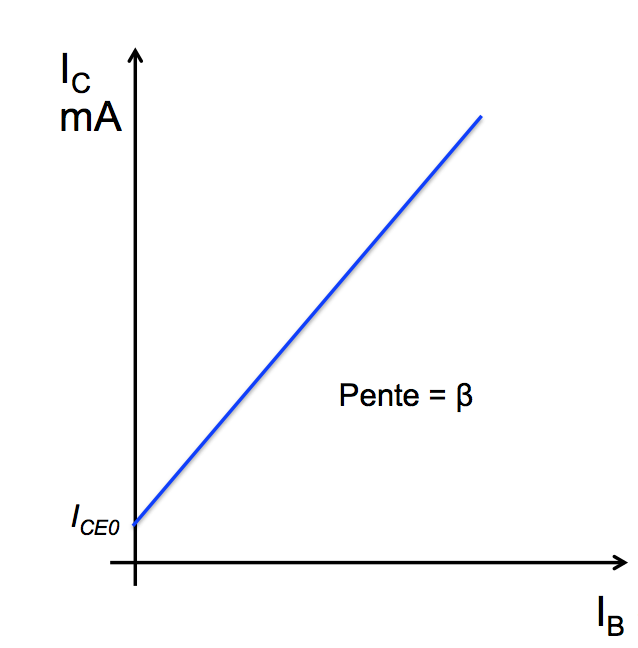
\includegraphics[scale=0.4]{Ic_Ib.png} 

Générateur de courant commandé par un courant. $I_{CE0}$ est le courant de fuite.
$$ 5< \beta < 80 : transistors\,de\,puissance \quad 100 < \beta < 500 : transistors\,de\,signal $$
\subsubsection{$I_C = f(V_{CE})$}
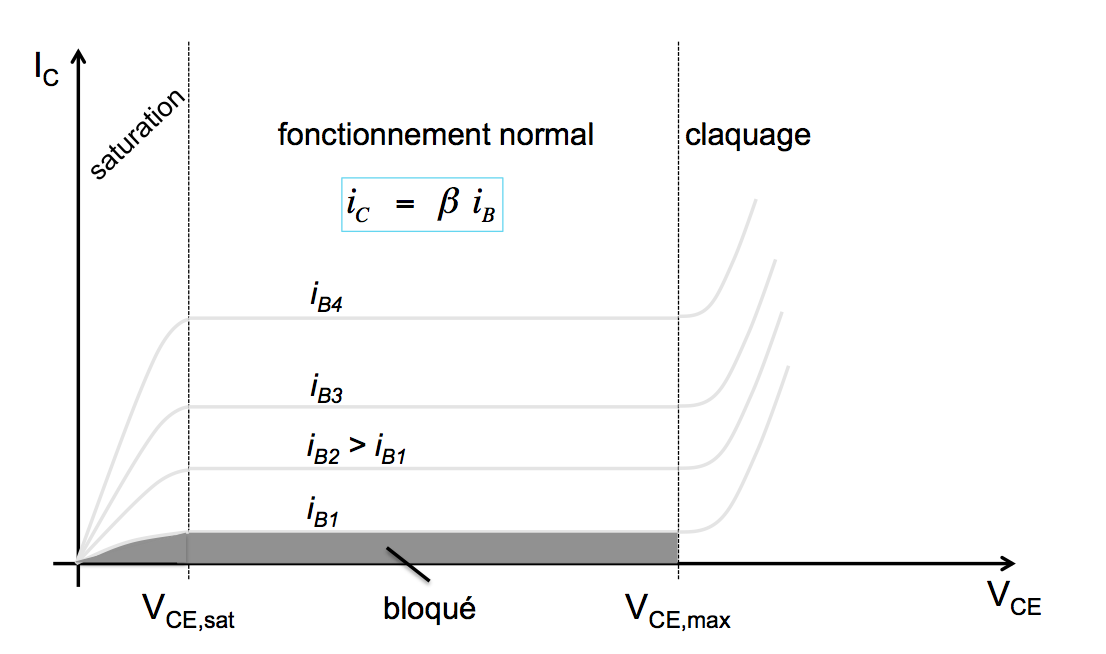
\includegraphics[scale=0.4]{Ic_Vce.png}

\subsubsection {Modèle grands signaux}
\begin{itemize}
\item \textbf{Blocage}$ V_{BE} < U_j ,\; I_C = 0A$
\item \textbf{Normal} 
\begin{itemize}
\item $V_{BE} = U_j , \; V_{BC} < U_j \;donc\; V_{CE}=V_{CB} + V_{BE} > 0 $

\item $I_C = \beta I_B $

\item $ I_E = (1+\beta)I_B \sim I_C $
\end{itemize}

\item \textbf{Saturation} 
\begin{itemize}
\item $ V_{BE} = V_{BC} = U_j \; donc\; V_{CE} = V_{CE,sat} \sim 0V$
\item $ I_B = I_{B,sat} > \frac{I_{C,sat}}{\beta} $ 
\end{itemize}
\end{itemize}

\subsubsection{Schémas équivalents}
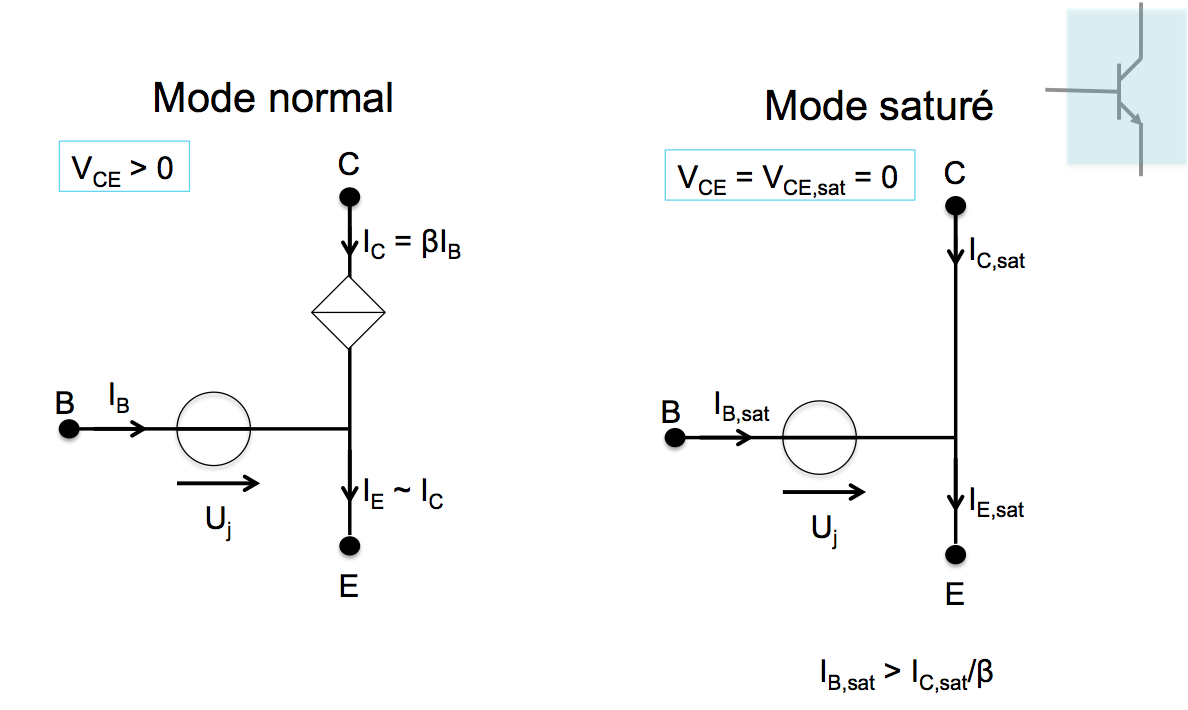
\includegraphics[scale=0.5]{schema_eq}
\subsection{Montage inverseur}
$V_X = V_{CC} - R_Ci_C$

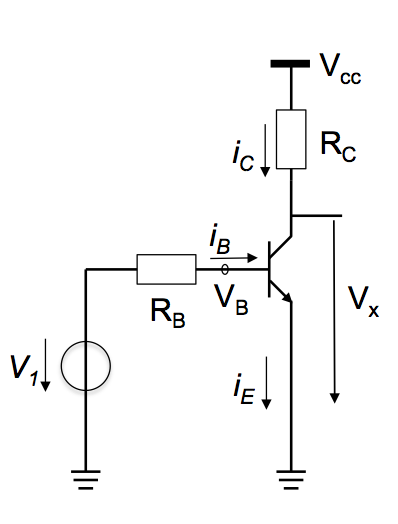
\includegraphics[scale=0.5]{inverseur}

\end{document}